%!TEX root = uist14.tex

\section{Iteration 2: Intensity IR}

\subsection{Problem Statement and Goal}
%With our first study, we learn that using IR to perform {\em coarse selection} can reduce the overall target selection time. A major reason for the improvement is because disambiguation is only needed 10\% of the time. 
%because in many cases there will be only one target in range and fine selection is not needed, and in cases where it’s needed, the list length has been effectively reduced. 
Performance of the {\em Naive IR} technique will degrade as target density in an environment increases, as increased density will require refinement steps. We therefore ask a follow-on research question: ``How might we improve selection time in a dense environment?''

\subsection{Technique}
Previously we only used IR reception as a binary signal for identifying potential targets. We hypothesize that IR intensity at the receiver side can provide more information about the likelihood that a user intended to select a particular target. Received IR intensity falls off with distance between IR emitter and receiver as well as with the angle between emitter and receiver. To measure intensity, we add an IR light-to-voltage converter (model number TSL267-LF from AMS-TAOS USA Inc and replace the IR emitter with IR emitter (model number SFH 4545 from OSRAM Opto Semiconductors Inc).
% transmitter webpage: http://www.digikey.com/product-search/en?x=0&y=0&lang=en&site=us&KeyWords=475-2919-ND
% http://www.digikey.com/product-detail/en/TSL267-LF/TSL267-LF-ND/3095052

We have empirically measured the intensity distribution at the receiver for this configuration in Figure~\ref{fig:measurement}. Our measurements confirm that angular difference has a large effect on the intensity readings (see how the IR intensity distribution changes when the offset from the center increases).

\begin{figure}[t]
\centering
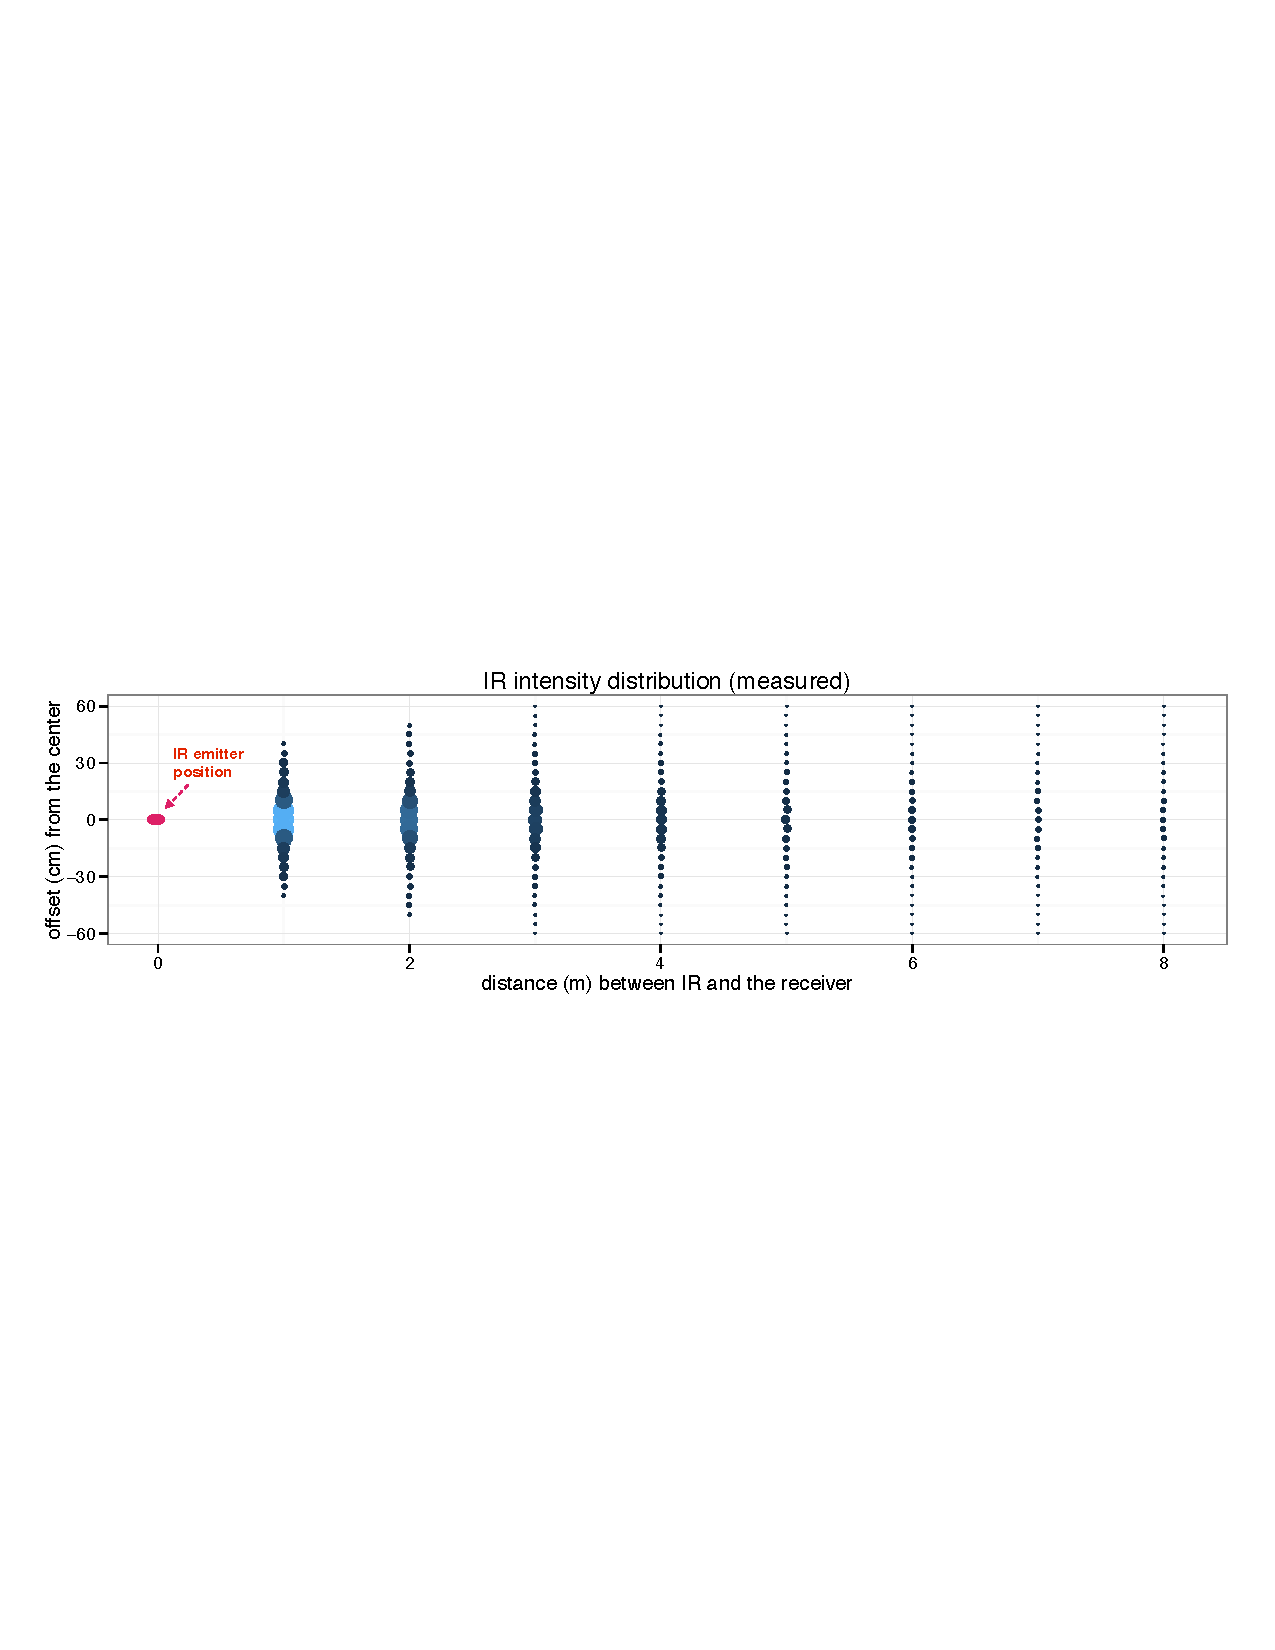
\includegraphics[width=1\columnwidth]{figures/IRIntensityDistribution.pdf}
\caption{Empirical measurement of IR intensity at different position. We measure the intensity at the plane of every 1 meter away from the IR emitter. On that plane, we obtain a sample every 5 centimeters. The size and color brightness in this graph represents the intensity readings.}
\label{fig:measurement}
\end{figure}

The intensity information is used in two ways:
\begin{enumerate}
\item When multiple targets have received IR signals and reported the intensity readings, we discard those whose intensities are significantly lower than the largest reading\footnote{In our current implementation, we empirically set it to be half of the ADC resolution, which is frequently used because it indicates a 3dB loss in the signal strength.}. Therefore, when there is only one target within line of sight, the IR intensity approach has the same behavior as the previous iteration - no disambiguation is needed. When the environment turns denser, the new design can filter some peripheral targets out, reducing $P(refine)$, the likelihood of entering the refinement stage.
\item When refinement is still needed, meaning that multiple targets have relatively close intensity values, the system sorts the disambiguation list according to the IR intensity, from strongest to weakest. We hypothesize that this will reduce time $t_{refine}$ significantly by minimizing extra navigation steps. (Ideally, the first list item will match the actual, intended target.)
\end{enumerate}

\subsection{Method}
To quantify the improvement this design we performed a second study to compare the {\em Naive IR} and {\em Intensity IR} approaches. Because we were interested in discovering performance differences in denser environment, we reposition the 10 nodes and set it up in a smaller area (see Figure~\ref{fig:study-layout2}) \bjoern{give measurements in meters}. We recruited 10 participants for this study. Each  user performed 30 target acquisition tasks for each approach. Similarly to our first within-subject study, half of them perform {\em Naive IR} first and the other half {\em Intesity IR} first.

\begin{figure}[t]
\centering
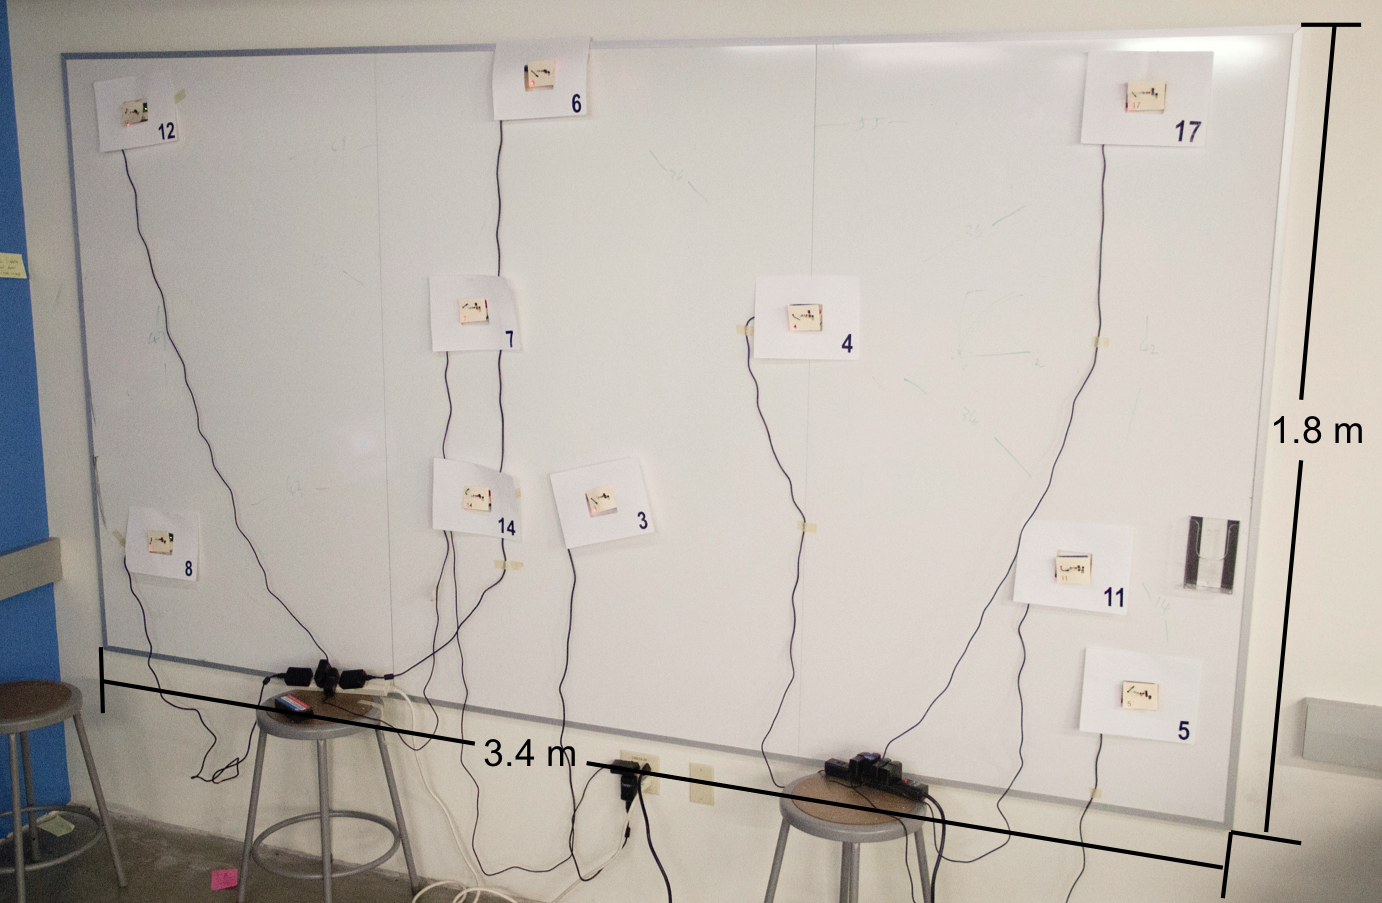
\includegraphics[width=1.0\columnwidth]{figures/study-layout2.png}
\caption{The environment setup for our second study. In comparison to our first study, we have delibrately increased the target density.}
\label{fig:study-layout2}
\end{figure}

% new study results
% ceiling(c(nrow(name), nrow(name_multiple), wrong_guess, wrong_percentage * 100))
% intensity
%  300 167  74  45
% name
%  300 225 145  65

%% first one
%% 
%             Outcome 1	Outcome 2	     Total
% Group 1 	167	133	300
% Group 2	225	75	300
% Total	        392	208	600
%% Chi squared equals 24.755 with 1 degrees of freedom. 
%%  The two-tailed P value is less than 0.0001


% 	    Outcome 1	Outcome 2	     Total
% Group 1	74	93	167
% Group 2	145	80	225
% Total	        219	173	392
% Chi squared equals 15.758 with 1 degrees of freedom. 
%   The two-tailed P value is less than 0.0001




\subsection{Results}
{\em Intensity IR} reduces the number of trials in which refinement dialogs are needed from 225 of 300 in {\em Naive IR} to 167 of 300 trials. A Chi-square test shows this difference is significant ($\chi^2(1) = 24.755$, $p < 0.0001$). This demonstrates that the new approach successfully reduces the probability that a disambiguation dialog is needed.

In the cases when disambiguation is inevitable, {\em Intensity IR} sorts the list based on the intensity reading, while {\em Naive IR} sorts alphabetically. {\em Intensity IR} reduces the fraction of refinement trails in which additional list navigation is necessary (i.e., the first, already selected element is incorrect).  {\em Intensity IR} sorted the desired target as the first one in the list in 55\% of cases (93 of 167). In comparison, for {\em Naive IR}, only 35\% of trials sorted the desired target as the first one in the list (80 out of 225). Again, a Chi-square test show that this difference is significant (with $\chi^2(1) = 15.758$, $p < 0.0001$. 

From Figure~\ref{fig:study2}, we can see that the overall target aquisition time has decreased from 4.31 seconds for {\em Naive IR} to 3.64 second for {\em Intensity IR}. This difference is also significant ($t(555)=3.2945$, $p=0.001$.) 

%  t.test(name$complete, intensity$complete)

% 	Welch Two Sample t-test

% data:  name$complete and intensity$complete
% t = 3.2945, df = 555.272, p-value = 0.001049
% alternative hypothesis: true difference in means is not equal to 0
% 95 percent confidence interval:
%  0.2707875 1.0704747
% sample estimates:
% mean of x mean of y 
%  4.311340  3.640709 

\begin{figure}[t]
\centering
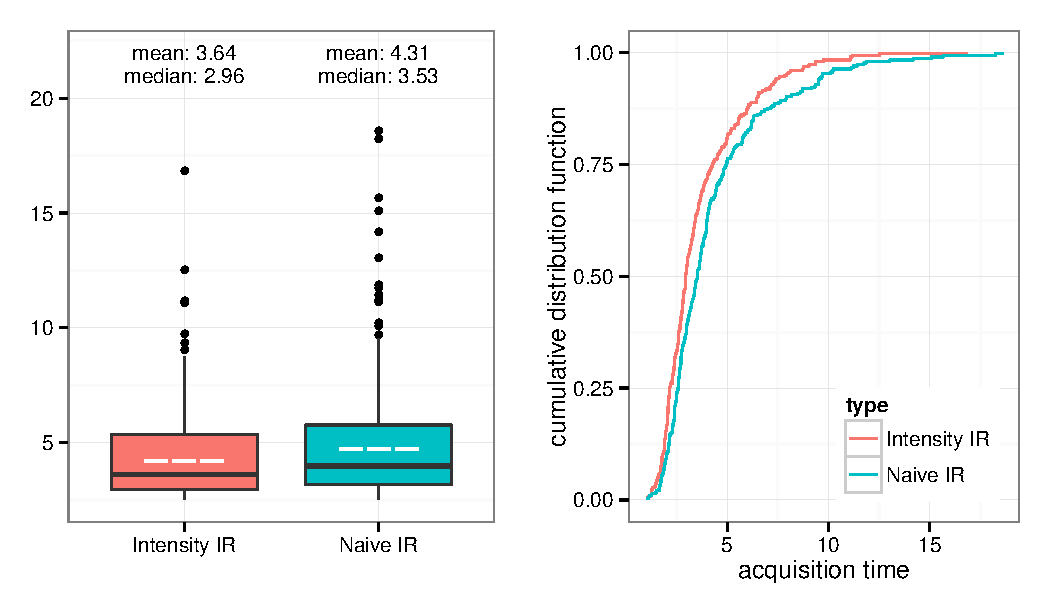
\includegraphics[width=1.0\columnwidth]{figures/result_study2.pdf}
\caption{Boxplot and CDF of the target acquisition time in {\em Naive IR} and {\em Intensity IR} conditions.}
\label{fig:study2}
\end{figure}

One side effect that we have observed in this approach is that the {\em Intensity IR} sometimes eliminates the desired target during the {\em scanning} stage. Out of 300 trials, 13 of them (4.3\%) has been accidentally eliminated. This is higher than the error rate for {\em Naive IR} (only 5 out of 300, ~1.6\%). % but this is the trade-off for the overall faster acquisition time.

%%% Local Variables: 
%%% mode: latex
%%% TeX-master: "uist14"
%%% End: 
